% ---------------------------------------------------------------------
% Das Dokument kompiliert mit pdflatex und ist auf Basis 
% von Koma-Script entstanden. 
%
% Autor des Templates (für Anmerkungen): 
% Michael von Riegen, riegen@informatik.uni-hamburg.de
%
% Einzelne Code-Teile für das Titelblatt sind aus dem Template 
% von Benjamin Kirchheim entnommen.
% Neue Titelseite von Josef Holnburger
%
% 25.05.09, Frank Langanke: Vorlage auf aktuelle KOMA-Version aktualisiert
% 26.05.09, Michael von Riegen: Anmerkung --> aktuelles Koma-Script ist nötig!
% 17.10.2016 neues Uni logo
% 21.08.2018 biblatex und scrlayer-scrpage statt scrpage2, anpassen auf SoWi-Layout
% ---------------------------------------------------------------------

% Wir nutzen Biblatex und biber für das Literaturverzeichnis
\documentclass[12pt, twoside = false, bibliography=totoc]{scrbook}
\usepackage[backend=biber, style=authoryear]{biblatex}
\addbibresource{bib.bib}

% Daten der Hausarbeit
% Bitte füllen Sie die folgenden Daten vollständig aus
\newcommand\myName{Josef Holnburger}
\newcommand\myStreetAddress{XXX}
\newcommand\myCityAddress{XXX}
\newcommand\myEmail{josef@holnburger.com}
\newcommand\myKeywords{Emotionen, Facebook, Wutbürger, Wahlkampf, Rechtspopulismus} % Optional
\newcommand\myMatNr{XXX}
\newcommand\myTitle{Musterhausarbeit}
\newcommand\mySubTitle{Mit einem besonders interessanten Untertitel}
\newcommand\thesisType{Hausarbeit}
\newcommand\fachbereich{Sozialwissenschaften} 
\newcommand\fachgebiet{Politikwissenschaft}
\newcommand\courseOfStudies{Musterseminar}
\newcommand\supervisorType{Dozentin} % Dozent*in, Seminarleiter etc.
\newcommand\supervisor{Lisa Musterfrau}
\newcommand\currentSemester{Wintersemester 2017/18}
\newcommand\dateOfSubmission{03.03.2018}

% Import von Paketen und Optionen die das gesamte Dokument betreffen
% sind in myPreamble.sty ausgelagert.
\usepackage{myPreamble}
   
\begin{document}


% TITELSEITE
% *************************************************************************
% *    Thesis / Dissertation Latex Template                                        
% *    
% *    Author: Leonard Heilig <leonard.heilig@uni-hamburg.de>
% *    modified by: Josef Holnburger <josef@holnburger.com>
% *   
% *    Note: some parts of this template are based on the VSIS template
% *              of Michael von Riegen <riegen@informatik.uni-hamburg.de>
% *   
% *************************************************************************

\begin{titlepage}

% START PAGE: -1
\setcounter{page}{-1}    

\begin{figure}[h]
	\begin{minipage}[t]{8.5cm}
	\flushleft 
			%Presented by: \> \textbf{\myName} \\
			%\> \textrm{\myAddress} \\
			%\> \textrm{\myEmail} \\
			Universität Hamburg \\
			Fachbereich: \fachbereich \\
			Fachgebiet: \fachgebiet \\
			Seminar: \courseOfStudies \\ 
			\supervisorType: \supervisor \\
			\currentSemester \\
	\end{minipage}
	\hfill
   \begin{minipage}[t][2cm][b]{0.35\textwidth}
    \flushright\noindent
    	\noindent
\includegraphics[scale=0.3]{images/UHH-Logo_2010_Farbe_CMYK.pdf}
    \end{minipage}
\end{figure}

\vspace*{\fill}
\begin{center}
	% THESIS TYPE
	\vspace{1cm}\noindent {\textbf{\thesisType}} \vspace{0.2cm} \\
	% THESIS TITLE
	\textbf{\Large \myTitle} \\
	\textbf{\mySubTitle} \\
	\dateOfSubmission \\
\end{center}
\vspace*{\fill}

\vspace*{\fill}%
\begin{figure}
	\myName \\
	Matrikelnummer:  \myMatNr \\
	\myStreetAddress \vspace{0.1cm} \\ 
	\myCityAddress \vspace{0.1cm}  \\
	E-Mail: \myEmail \\ 
\end{figure}

\end{titlepage}



% VERZEICHNISSE (Inhaltsverzeichnis, Abkürzungen)
% Vorspann einleiten --> Seitennummerierung römisch
\frontmatter

% Inhaltsverzeichnis
\tableofcontents

% Abbildungs- und Tabllenverzeichnis auf einer Seite
\listoffigures
\addcontentsline{toc}{chapter}{\listfigurename}
\vspace*{24pt}
{\let\clearpage\relax \listoftables}	
\addcontentsline{toc}{chapter}{\listtablename}

% Hauptteil einleiten --> Seitennummerierung wieder arabisch
\mainmatter

\chapter{Einleitung}\label{Einleitung}

Hier kommt eine Quellenangabe \parencite{bartlett_populism_2014}. Weiterhin sieht man hier einen Link auf Abbildung \ref{fig:Übersicht_Parteien_2013-17}. Lorem ipsum dolor sit amet, consectetuer\footnote{Hier ist eine Fußnote!} adipiscing elit \parencite[vgl.][]{bobba_age_2017}. 
\blindtext

\vspace*{4pt}
\begin{figure}[h]
	\centering
		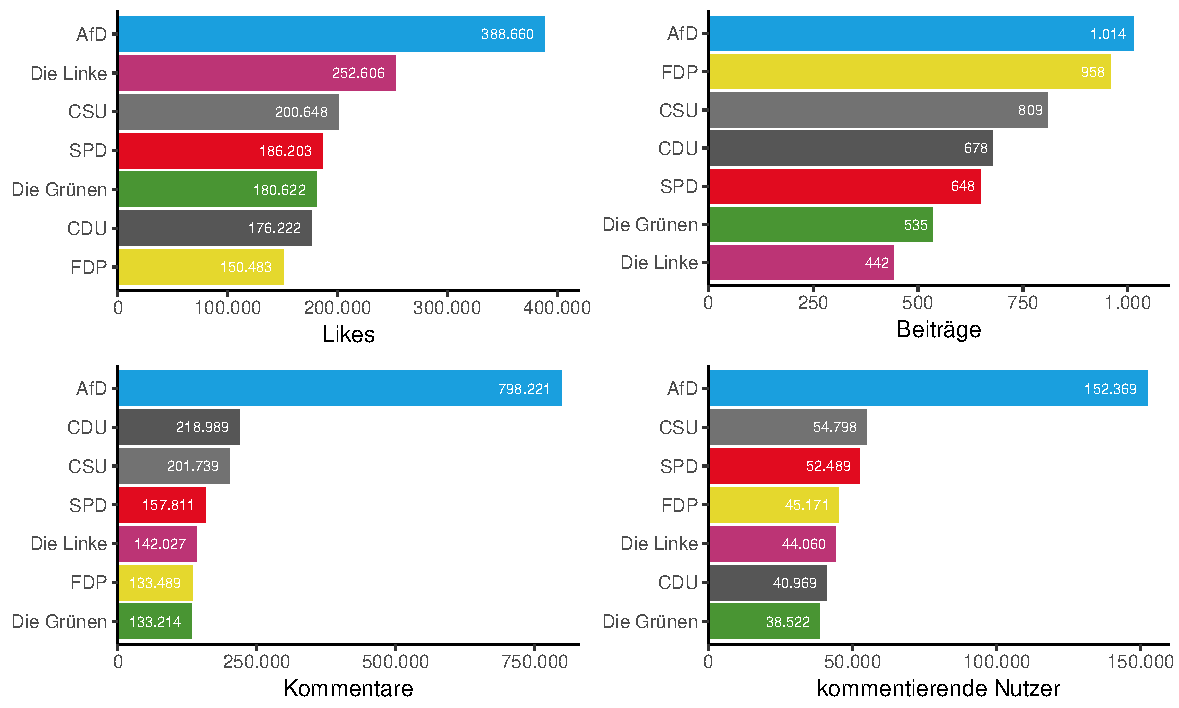
\includegraphics[width=1.0\textwidth]{plots/overview_posts_user_2017}
	\caption[Übersicht der Likes, Anzahl der Beiträge, Kommentare und kommentierenden Nutzer auf den Facebookseiten der Parteien]{Übersicht der Likes, Beiträge, Kommentare und kommentierenden Nutzer der Facebookseiten der Parteien. Auswertungszeitraum: 01.01.2017 bis 31.12.2017}
	\label{fig:Übersicht_Parteien_2013-17}
\end{figure}

\blindtext

\blindtext

\blindtext \parencite[vgl.][S.12]{forchtner_mediatization_2013}

\blinddocument

\section{Facebook und die Parteien}

\blindtext

\captionsetup{justification=raggedright}
% latex table generated in R 3.4.3 by xtable 1.8-2 package
% Sat Mar  3 21:30:03 2018
\begin{table}[ht]
\centering
\caption[Summe der Reaktionen auf Beiträge der Parteien]{Summe der Reaktionen auf Beiträge der Parteien (01.03.2016 bis 31.12.2017)} 
\label{tab_Reactions}
\begin{tabular}{lrrrrrr}
  \hline
Partei & Love & Haha & Wow & Traurig & Wütend & Summe \\ 
  \hline
AfD & 126.610 & 249.089 & 31.561 & 77.289 & 624.391 & 1.108.940 \\ 
  CSU & 31.110 & 115.891 & 10.783 & 23.111 & 72.096 & 252.991 \\ 
  Die Linke & 42.940 & 13.974 & 3.953 & 17.314 & 34.615 & 112.796 \\ 
  SPD & 42.018 & 31.928 & 4.025 & 17.121 & 16.565 & 111.657 \\ 
  CDU & 28.403 & 30.025 & 2.001 & 6.832 & 16.661 & 83.922 \\ 
  Die Grünen & 27.751 & 20.168 & 2.569 & 13.956 & 16.702 & 81.146 \\ 
  FDP & 28.094 & 15.336 & 3.611 & 11.224 & 11.160 & 69.425 \\ 
   \hline
\end{tabular}
\end{table}
 

\chapter{Reaktionen}

\blindtext


\printbibliography[title={Literaturverzeichnis}]

    
\end{document}